%%%% Proceedings format for most of ACM conferences (with the exceptions listed below) and all ICPS volumes.
\documentclass[sigconf]{acmart}
%%%% As of March 2017, [siggraph] is no longer used. Please use sigconf (above) for SIGGRAPH conferences.

%%%% Proceedings format for SIGPLAN conferences 
% \documentclass[sigplan, anonymous, review]{acmart}

%%%% Proceedings format for SIGCHI conferences
% \documentclass[sigchi, review]{acmart}

%%%% To use the SIGCHI extended abstract template, please visit
% https://www.overleaf.com/read/zzzfqvkmrfzn


\usepackage{booktabs} 	% For formal tables
\usepackage{indentfirst}% For indenting first paragraphs

% --------------------------- LATER --------------------------------------


% Copyright 
% I don't know what our copyright is on this?
%\setcopyright{none}
%\setcopyright{acmcopyright}
%\setcopyright{acmlicensed}
\setcopyright{rightsretained}
%\setcopyright{usgov}
%\setcopyright{usgovmixed}
%\setcopyright{cagov}
%\setcopyright{cagovmixed}


% DOI
%\acmDOI{10.475/123_4}

% ISBN
%\acmISBN{123-4567-24-567/08/06}

%Conference
%\acmConference[WOODSTOCK'97]{ACM Woodstock conference}{July 1997}{El
  %Paso, Texas USA}
%\acmYear{1997}
%\copyrightyear{2016}


%\acmArticle{4}
%\acmPrice{15.00}
% ------------------------------------------------------------------------

\begin{document}
\title{Temp Title: Non-Functional Bugs Project}
%\titlenote{Produces the permission block, and copyright information}

\author{Aida Radu}
\affiliation{
  \institution{Dept. of Computing Science \\ University of Alberta}
  \city{Edmonton}
  \state{Canada}
}
\email{aradu@ualberta.ca}

\author{Sarah Nadi}
\affiliation{
  \institution{Dept. of Computing Science \\ University of Alberta}
  \city{Edmonton}
  \country{Canada}
}
\email{nadi@ualberta.ca}


\begin{abstract}
[PLACEHOLDER TEXT]

\end{abstract}

% The code below should be generated by the tool at
% http://dl.acm.org/ccs.cfm

\begin{CCSXML}
	<ccs2012>
	<concept>
	<concept_id>10011007</concept_id>
	<concept_desc>Software and its engineering</concept_desc>
	<concept_significance>500</concept_significance>
	</concept>
    
	<concept>
	<concept_id>10011007.10010940.10011003</concept_id>
	<concept_desc>Software and its engineering~Extra-functional properties</concept_desc>
	<concept_significance>500</concept_significance>
	</concept>
	</ccs2012>
\end{CCSXML}

\ccsdesc[500]{Software and its engineering}
\ccsdesc[500]{Software and its engineering~Extra-functional properties}


\keywords{Repository Mining; Bug Detection}


\maketitle

% ---------------------------------------------------------------------------------------------------
\section{Introduction}
% ---------------------------------------------------------------------------------------------------
\section{Background}
% ---------------------------------------------------------------------------------------------------
\section{Methodology}
To create our dataset, we looked at a variety of Github repositories written in either Java or Python. 
We used two main methods to identify candidate repositories for mining. 
 
\subsection{Initial Procedure}
First, we used the Github API to search for projects written in Java or Python, and sorted them based on their number of stars. We then selected the top 90 repositories from these results. 

\subsubsection{Obtaining commits}
To extract commits related to non-functional requirements, we implemented a keyword search using PyDriller \footnote{https://github.com/ishepard/pydriller, Davide Spadini 2018}. The stemmed keywords are listed in Table \ref{tab:kwds}. Example word endings are in square brackets.

% --------------- TABLE -------------
\begin{table}
  \caption{Commit Message Keywords}
  \label{tab:kwds}
\begin{tabular}{ c c c }
  \toprule
   "fix"             &"bug"           &"error"\\
   "refactor"	     &"secur[ity]"    &"maint[enance]"\\
   "stab[ility]"     &"portab[ility]" &"efficien[cy]"\\
   "usab[ility]"     &"reliab[ility]" &"testab[ility]"\\
   "changeab[ility]" &"replace"       &"memory"\\
   "resource"        &"runtime"       &"crash"\\
   "leak"            &"attack"        &"authenticat[ion]"\\
   "authoriz[ation]" &"cipher"        &"crack" \\ 
   "decrypt"         &"encrypt"       &"vulnerab[ility]"\\ 
   "minimize"        &"optimize"      &"slow"\\
   "\#"              &                &\\
  \bottomrule
\end{tabular}
\end{table}
% --------------- TABLE -------------

For those repositories identified by star rating, we directly ran PyDriller; note that some of these projects contained zero true positives. 
Our PyDriller program mined the commit history of each project, and outputted a CSV file containing the id and message of the commits containing one or more of the keywords in Table \ref{tab:kwds}. For projects written in Java, we further limited our search to commits affecting \texttt{.java} files. Likewise, for Python projects, we looked at \texttt{.py} files.

We then manually searched these files for true positives. We ignored commits that, despite containing one or more of the keywords in our list, did not relate to non-functional requirements (e.g., ``Fix copy paste error''\footnote{https://github.com/jenkinsci/jenkins/commit/9fb6ccf} and ``Allow modules to replace visual character representation''\footnote{https://github.com/MovingBlocks/Terasology/commit/45f915a}). Furthermore, we did not include problems that were highly specific to the given project. 


\subsection{Alternate Procedure}
Using our first method, we found several instances where developers corrected memory leaks, or replaced one API with another to improve performance. Thus, for our second method, we identified candidate repos using Github`s search bar to find similar changes. We searched for commits containing the keywords in Table \ref{tab:kwds}. As well, we searched for language-specific enhancements such as ``StringBuilder replace,'' and ``foreach loop replace.'' We documented the bug that was found in the search, then ran PyDriller on the complete repo history. Thus, these projects always had at least one true positive. Once we ran PyDriller, the method was identical to that in the previous section.

\subsection{Documentation} 
For each problem we identified, we recorded the problem meta data in a YAML\footnote{http://yaml.org/, last checked on June 27, 2018} file. Figure \ref{fig:meta1} shows an example of our format. Each file specifies the problem's \texttt{source}. The source \texttt{commit-msg-keywords} refers to method one, while \texttt{github-search} refers to method two. Under the \texttt{project} field, we specify the \texttt{name} of the project and the \texttt{url} of its Github repository. We also document the \texttt{commit url} and \texttt{commit message} associated with the fix, as well as the particular \texttt{file} and \texttt{method} affected. Because a user`s commit message is not always thorough, we construct a \texttt{description} of our interpretation of the problem.

In addition, we assign on or more tags to each problem according to the type of fix. Our collection of tags consists of: \texttt{security}, \texttt{performance}, \texttt{memory}  and \texttt{resource management}. For fixes related to specific APIs (e.g., using a StringBuilder in place of  a String), we record the involved \texttt{API}, as well as a \texttt{rule} corresponding to the change. For commits not connected to a particular API, we create a general \texttt{suggestion} to address similar problems. An example of this type is shown in Figure \ref{fig:meta2}. 

% --------------- FIGURE -------------
\begin{figure}
  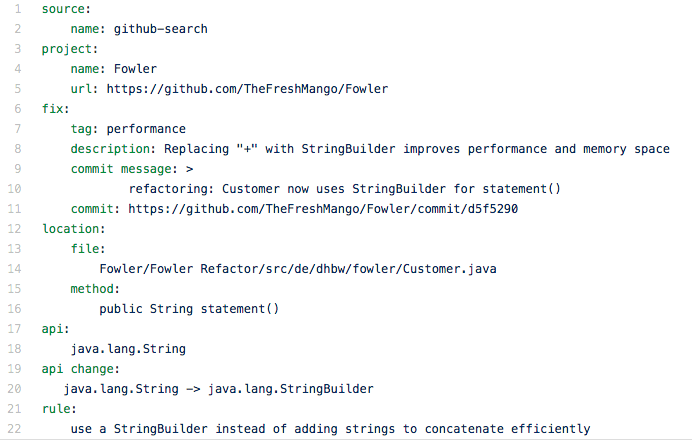
\includegraphics[height=2in, width=3in]{YAMLmetadata}
  \caption{Meta Data for \texttt{Fowler} - problem 2}
  \label{fig:meta1}
\end{figure}
% --------------- FIGURE -------------


% --------------- FIGURE -------------
\begin{figure}
  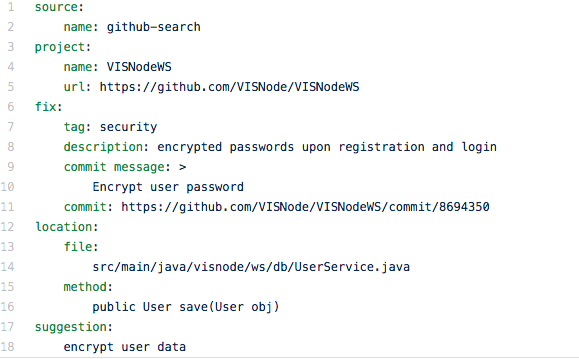
\includegraphics[height=2in, width=3in]{YAMLmetadata2}
  \caption{Meta Data for \texttt{VISNodeWS} - problem 1}
  \label{fig:meta2}
\end{figure}
% --------------- FIGURE -------------

% ---------------------------------------------------------------------------------------------------
\section{Dataset}

Using the first procedure, we mined 90 Java repositories and 15 Python repositories. Of these, 16 Java and 8 Python repositories contained true positives. In total, we identified 62  problems using this method. Using the second procedure, we obtained 32 problems from 18 Java repositories and 13 Python repositories. The distribution of problems by type and language is shown in Table \ref{tab:type}.

% --------------- TABLE -------------
\begin{table}
  \caption{Data Distribution}
  \label{tab:type}
\begin{tabular}{ c c c c }
  \toprule
  Problem Type & Python & Java & Total\\
  \midrule
  API        		&	17  &  44 &  62\\
  General    		&	12  &  17 &  31\\
  Project Specific  	&	1  &   3 &    4\\
  \midrule
  Total      		&	30  &  64 &  94\\
  \bottomrule
\end{tabular}
\end{table}
% --------------- TABLE -------------

The number of problems per tag are displayed in \ref{tab:tag}. Performance related bugs were the most common subtype. Table \ref{tab:domain} shows the number of projects in our dataset that have stars,watches, and forks within a given range. Nineteen of the projects had no stars; all of these were identified via the \texttt{github-search} procedure.

% because some have two tags, this has to be a separate table, otherwise the totals wouldn't add up
% --------------- TABLE -------------
\begin{table}
  \caption{Data Distribution by Problem Tag}
  \label{tab:tag}
\begin{tabular}{  c c c c }
  \toprule
  Tag  		 	&Python &Java & Total\\
  \midrule
  security		& 9 &16 &25 \\
  performance		&12 &30 &42 \\
  memory		& 4 &23 &27 \\
  resource management	& 1 & 5&  6 \\
  \bottomrule
\end{tabular}
\end{table}
% --------------- TABLE -------------

% --------------- TABLE -------------
\begin{table}
  \caption{Number of Projects by Github Stats}
  \label{tab:domain}
\begin{tabular}{ c c c c }
  \toprule
  Range & stars & watches & forks\\
  \midrule
  0		&19 & 7& 23\\
  1-100		&12 &42& 21\\
  101-500	&13 & 8& 10\\
  501-1000	& 8 & 2&  0\\
  >1000   	& 8 & 1&  6\\
  \bottomrule
\end{tabular}
\end{table}
% --------------- TABLE -------------

% ---------------------------------------------------------------------------------------------------
\section{Discussion and Directions for Future Work}
% ---------------------------------------------------------------------------------------------------
\section{Conclusions}
% ---------------------------------------------------------------------------------------------------
\section*{Threats to Validity}
% ---------------------------------------------------------------------------------------------------
\section*{Acknowledgements}


\bibliographystyle{ACM-Reference-Format}
\bibliography{bibRaduNadi2018}

\end{document}

